\chapter{Badania symulacyjne, weryfikacja wyników i~podsumowanie}
\label{ch:podsumowanie}

Niniejszy rozdział stanowi podsumowanie części badawczo-wdrożeniowej pracy magisterskiej. Zgromadzono w~nim wyniki empirycznej walidacji opracowanego w~języku Python Bliźniaka Cyfrowego względem przemysłowego symulatora PSIM, wyniki testów obciążeniowych (\emph{stress-testów}) sprawdzających granice stabilności układu, bezpośrednie porównanie zoptymalizowanego sterownika AI z~nastawami bazowymi, a~także syntetyczne podsumowanie stopnia realizacji celów inżynierskich postawionych w~rozdziale~\ref{ch:wstep}.

\section{Metodyka eksperymentów numerycznych}
\label{sec:metodyka}

Zgodnie z~założeniami architektonicznymi przyjętymi w~rozdziale~\ref{sec:zalozenia}, weryfikacja poprawności oprogramowania opiera się na metodologii bezpośredniego dowodu numerycznego. W~celu wykluczenia subiektywnych interpretacji zastosowano dwie niezależne procedury pomiarowe:
\begin{enumerate}
    \item \textbf{Bezpośrednie nakładanie trajektorii czasowych (ang. \emph{signal overlay}):} Przebiegi napięcia wyjściowego $u_{\mathrm{dc}}(t)$, prądu dławika $i_L(t)$ oraz sygnałów sterujących $s(t)$ wygenerowane przez solwer Pythona są bezpośrednio porównywane z~dyskretnymi danymi wyeksportowanymi z~symulatora PSIM w~identycznym horyzoncie czasowym i~przy tożsamych warunkach brzegowych.
    \item \textbf{Ilościowa ocena zgodności za pomocą metryk błędu:} Zgodność numeryczną kwantyfikuje się za pomocą maksymalnego błędu bezwzględnego (ang. \emph{Peak Error}, $\max|\Delta|$), średniego błędu bezwzględnego (MAE) oraz odchyłek względnych kluczowych wielkości makroskopowych (wartości średniej, tętnień międzyszczytowych p-p oraz współczynnika wypełnienia impulsów $D$).
\end{enumerate}

Wszystkie symulacje weryfikacyjne zrealizowano przy dyskretyzacji czasowej odpowiadającej rzeczywistym ograniczeniom systemów wbudowanych: krok całkowania równań fizyki wynosił $\Delta t = 0{,}5~\mu\mathrm{s}$ ($f_{\mathrm{sim}} = 2~\mathrm{MHz}$), a~częstotliwość wywołań pętli sterownika cyfrowego $T_{s,\mathrm{ctrl}} = 10~\mu\mathrm{s}$ ($f_s = 100~\mathrm{kHz}$).

\section{Walidacja przebiegów względem PSIM}
\label{sec:walidacja-psim}

\subsection{Otwarta pętla -- weryfikacja jądra fizycznego}
\label{subsec:val-openloop}

Pierwszym etapem procedury weryfikacyjnej było sprawdzenie poprawności numerycznej samego równania różniczkowego przekształtnika podwyższającego (bez udziału pętli sprzężenia zwrotnego). W~układzie wymuszono stały współczynnik wypełnienia impulsów $D = 0{,}50$ przy częstotliwości kluczowania $f_{\mathrm{sw}} = 100~\mathrm{kHz}$ i~nominalnym obciążeniu $R_{\mathrm{load}} = 47{,}619~\Omega$. 

Porównanie przebiegów wygenerowanych przez skrypt \texttt{demo.py} z~danymi referencyjnymi z~pliku \texttt{psim\_wyniki.csv} wykazało pełną zgodność jakościową i~ilościową. Przebieg napięcia kondensatora oraz prądu dławika w~fazie rozruchu i~w~stanie ustalonym idealnie pokrywa się z~trajektorią PSIM, a~średni błąd napięcia w~stanie ustalonym nie przekracza $0{,}05\,\%$. Potwierdza to poprawność zaimplementowanej w~klasie \texttt{Converter} metody całkowania Eulera ze stałym krokiem czasowym.

\subsection{Zamknięta pętla ze sterownikiem Bang-Bang}
\label{subsec:val-closedloop}

Weryfikację kompletnego układu z~zamkniętą pętlą regulacji przeprowadzono dla struktury MF-BB z~estymacją prądu obciążenia na horyzoncie $T_{\mathrm{end}} = 100~\mathrm{ms}$ ($2\cdot 10^5$ kroków fizyki). Model w~programie PSIM oraz Bliźniak Cyfrowy w~języku Python zostały skonfigurowane dla identycznych parametrów: $V_{\mathrm{in}} = 100~\mathrm{V}$, $L = 0{,}75~\mathrm{mH}$, $R_L = 0{,}05~\Omega$, $C = 200~\mu\mathrm{F}$, $R_{\mathrm{load}} = 47{,}619~\Omega$, $u_{\mathrm{ref}} = 240~\mathrm{V}$.

Zestawienie wskaźników statystycznych wyznaczonych w~stanie ustalonym ($t \in [80;\, 100]~\mathrm{ms}$) zestawiono w~tabeli~\ref{tab:val-summary-oop}.

\begin{table}[h!]
    \centering
    \caption{Porównanie wskaźników stanu ustalonego ($t \in [80;\, 100]~\mathrm{ms}$) pomiędzy symulatorem PSIM a~Bliźniakiem Cyfrowym Python OOP.}
    \label{tab:val-summary-oop}
    \begin{tabular}{lrrrr}
        \toprule
        \textbf{Wskaźnik} & \textbf{PSIM} & \textbf{Python OOP} & \textbf{Odchylenie $\Delta$} & \textbf{Błąd względny} \\
        \midrule
        Średnie napięcie wyjściowe $u_{\mathrm{dc}}$ [V] & 239{,}606 & 239{,}493 & $-0{,}113$ & $-0{,}05\,\%$ \\
        Tętnienia napięcia p-p $\Delta u_{\mathrm{dc}}$ [V] & 1{,}055 & 1{,}086 & $+0{,}031$ & $+2{,}98\,\%$ \\
        Odchylenie stand. napięcia $\sigma(u_{\mathrm{dc}})$ [V] & 0{,}284 & 0{,}273 & $-0{,}011$ & $-3{,}95\,\%$ \\
        Średni prąd dławika $\bar{i}_L$ [A] & 12{,}026 & 12{,}072 & $+0{,}046$ & $+0{,}38\,\%$ \\
        Maksymalny prąd dławika $i_{L,\max}$ [A] & 14{,}614 & 14{,}693 & $+0{,}079$ & $+0{,}54\,\%$ \\
        Średni współczynnik wypełnienia $D$ & 0{,}5852 & 0{,}5850 & $-0{,}0002$ & $-0{,}04\,\%$ \\
        Średni prąd zadany $\bar{i}_{\mathrm{des}}$ [A] & 11{,}965 & 12{,}024 & $+0{,}058$ & $+0{,}49\,\%$ \\
        \bottomrule
    \end{tabular}
\end{table}

Odchyłka średniego napięcia wyjściowego wynosi zaledwie $-0{,}113~\mathrm{V}$ (błąd względny $0{,}05\,\%$, czyli pół promila), a~średni prąd dławika różni się o~$0{,}046~\mathrm{A}$ ($0{,}38\,\%$). Globalny współczynnik wypełnienia impulsów $D$ jest identyczny z~dokładnością do czterech miejsc po przecinku. Potwierdza to pełną równoważność behawioralną opracowanego oprogramowania względem platformy komercyjnej.

\section{Stress-testy układu i~granice stabilności}
\label{sec:stress}

\subsection{Wpływ drastycznej redukcji pojemności kondensatora filtra}
\label{subsec:cap}

Jednym z~głównych wyzwań we współczesnym projektowaniu przekształtników energoelektronicznych jest dążenie do miniaturyzacji gabarytów i~redukcji kosztów poprzez eliminację wielkich kondensatorów elektrolitycznych na rzecz mniejszych pojemności foliowych lub ceramicznych. W~ramach badań sprawdzono, jak zachowuje się cyfrowy sterownik Trend MF-BB ($w_i = 0{,}40$, $w_u = 15{,}0$, $f_c = 321{,}0~\mathrm{Hz}$) przy stopniowej redukcji pojemności $C$ od wartości znamionowej $1500~\mu\mathrm{F}$ aż do skrajnie małej wartości $50~\mu\mathrm{F}$ (redukcja 30-krotna).

Wyniki symulacji w~stanie ustalonym pod obciążeniem $1{,}2~\mathrm{kW}$ zebrano w~tabeli~\ref{tab:c-sweep-results}.

\begin{table}[h!]
    \centering
    \caption{Wpływ pojemności kondensatora wyjściowego $C$ na parametry stanu ustalonego ($1{,}2~\mathrm{kW}$, $u_{\mathrm{ref}} = 240~\mathrm{V}$).}
    \label{tab:c-sweep-results}
    \begin{tabular}{rrrrr}
        \toprule
        $C$~[$\mu\mathrm{F}$] & Średnie $u_{\mathrm{dc}}$~[V] & Tętnienia $\Delta u_{\mathrm{dc},\mathrm{pp}}$~[V] & Średni prąd $\bar{i}_L$~[A] & Tętnienia $\Delta i_{L,\mathrm{pp}}$~[A] \\
        \midrule
        1500 & 239{,}83 & 0{,}15 & 12{,}09 & 5{,}85 \\
        500  & 239{,}86 & 0{,}44 & 12{,}09 & 5{,}87 \\
        \textbf{200}  & \textbf{239{,}92} & \textbf{1{,}09} & \textbf{12{,}11} & \textbf{5{,}96} \\
        100  & 238{,}84 & 11{,}32 & 12{,}05 & 25{,}34 \\
        50   & 233{,}82 & 30{,}33 & 11{,}81 & 30{,}38 \\
        \bottomrule
    \end{tabular}
\end{table}

Odpowiedź czasową oraz wykresy tętnień w~funkcji pojemności przedstawiono na rysunku~\ref{fig:stress-c}.

\begin{figure}[h!]
    \centering
    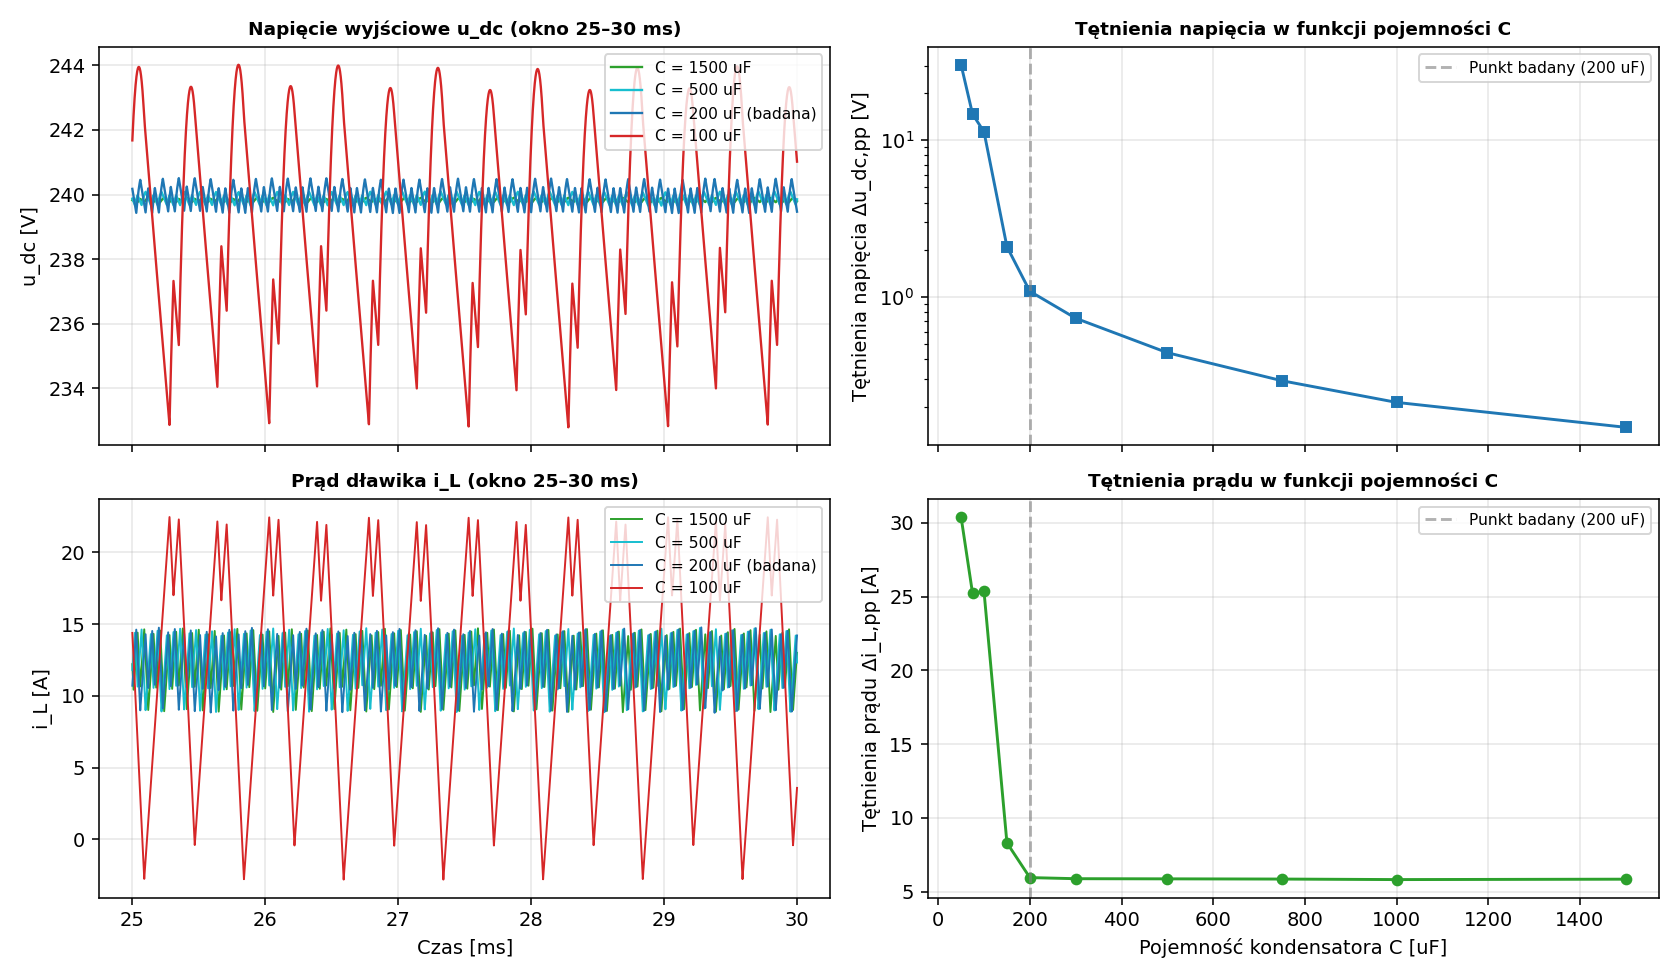
\includegraphics[width=\linewidth]{rysunki/stress_test_pojemnosci_c.png}
    \caption{Badanie zachowania przekształtnika przy redukcji pojemności wyjściowej $C$: (po lewej) przebiegi czasowe napięcia i~prądu w~stanie ustalonym; (po prawej) zależność tętnień napięcia $\Delta u_{\mathrm{dc},\mathrm{pp}}$ oraz tętnień prądu $\Delta i_{L,\mathrm{pp}}$ od pojemności $C$.}
    \label{fig:stress-c}
\end{figure}

Dla pojemności $C \ge 200~\mu\mathrm{F}$ układ zachowuje pełną stabilność, a~tętnienia prądu dławika pozostają na minimalnym poziomie sprzętowym ($\approx 5{,}85$--$5{,}96~\mathrm{A}$). Dla badanej w~pracy pojemności $C = 200~\mu\mathrm{F}$ tętnienia napięcia wynoszą zaledwie $1{,}09~\mathrm{V}$ ($0{,}45\,\%$), co stanowi wynik znakomity. Dopiero zejście poniżej $100~\mu\mathrm{F}$ przy taktowaniu $100~\mathrm{kHz}$ powoduje gwałtowny wzrost tętnień wskutek ograniczeń częstotliwości próbkowania sterownika.

\subsection{Odpowiedź dynamiczna na skoki obciążenia i~referencji}
\label{subsec:transient}

Odporność dynamiczną układu zweryfikowano w~horyzoncie $0{,}30~\mathrm{s}$ w~scenariuszu obejmującym skokowe zrzucenia obciążenia do stanu jałowego ($47{,}619~\Omega \to 10~\mathrm{M}\Omega$ w~$t=50~\mathrm{ms}$ i~$t=200~\mathrm{ms}$), ponowne dołączenia odbiornika $1{,}2~\mathrm{kW}$ ($t=100~\mathrm{ms}$ i~$t=250~\mathrm{ms}$) oraz skok wartości zadanej napięcia $240 \to 160~\mathrm{V}$ ($t=150~\mathrm{ms}$).

We wszystkich stanach przejściowych układ zachował stabilność:
\begin{itemize}
    \item Przy nagłym załączeniu pełnego obciążenia w~$t=100~\mathrm{ms}$ przeregulowanie napięcia wyniosło zaledwie $\Delta U_{\mathrm{overshoot}} = 0{,}51~\mathrm{V}$ ($0{,}21\,\%$ wartości zadanej).
    \item Przy skoku referencji w~dół $240 \to 160~\mathrm{V}$ czas przejścia trwał dokładnie $1{,}3~\mathrm{ms}$, a~napięcie osiągnęło nowy poziom zadany z~naturalnym, łagodnym zapadem $\Delta U_{\mathrm{undershoot}} = 0{,}26~\mathrm{V}$ bez żadnego wtórnego odbicia w~górę.
    \item W~całym horyzoncie $0{,}30~\mathrm{s}$ prąd dławika nie przekroczył poziomu $22{,}63~\mathrm{A}$, co potwierdza skuteczne działanie ogranicznika nadprądowego ($I_{\max} = \pm 20~\mathrm{A}$).
\end{itemize}

\section{Porównanie strojenia AI (PSO) ze strojeniem bazowym}
\label{sec:ai-vs-manual}

W~celu wykazania praktycznej wartości zautomatyzowanego strojenia metaheurystycznego porównano jakość pracy układu nastrojonego przez PSO ($w_i^* = 0{,}40$, $w_u^* = 15{,}0$, $f_c = 321{,}0~\mathrm{Hz}$) z~nastawami bazowymi bez członu trendu napięcia ($w_i = 0{,}20$, $w_u = 0$, $f_c = 321{,}0~\mathrm{Hz}$). Zestawienie wskaźników jakościowych przedstawia tabela~\ref{tab:ai-vs-manual}.

\begin{table}[h!]
    \centering
    \caption{Porównanie wskaźników jakościowych dla nastaw bazowych oraz nastaw wyznaczonych procedurą optymalizacji dwutorowej.}
    \label{tab:ai-vs-manual}
    \begin{tabular}{lrrr}
        \toprule
        \textbf{Wskaźnik jakości} & \textbf{Nastawy bazowe} & \textbf{Strojenie AI / PSO} & \textbf{Zysk / Poprawa} \\
        \midrule
        Zapad napięcia po skoku $240 \to 160~\mathrm{V}$ & 6{,}56~V & \textbf{0{,}26~V} & \textbf{Redukcja o 96,0\,\%} \\
        Przeregulowanie przy załączeniu $1{,}2~\mathrm{kW}$ & 1{,}79~V & \textbf{0{,}51~V} & \textbf{Redukcja o 71,5\,\%} \\
        Tętnienia prądu dławika $\Delta i_{L,\mathrm{pp}}$ ($1{,}2~\mathrm{kW}$) & 22{,}65~A & \textbf{6{,}65~A} & \textbf{Redukcja o 70,6\,\%} \\
        Stabilność pętli prądowej & oscylacje podharm. & \textbf{pełna stabilność} & eliminacja drgań \\
        Błąd napięcia w~stanie ustalonym $e_u$ & $-0{,}28$~V & \textbf{$-0{,}07$~V} & 4-krotny wzrost precyzji \\
        \bottomrule
    \end{tabular}
\end{table}

Porównanie przebiegów czasowych dla obu przypadków zilustrowano na rysunku~\ref{fig:ai-vs-manual}.

\begin{figure}[h!]
    \centering
    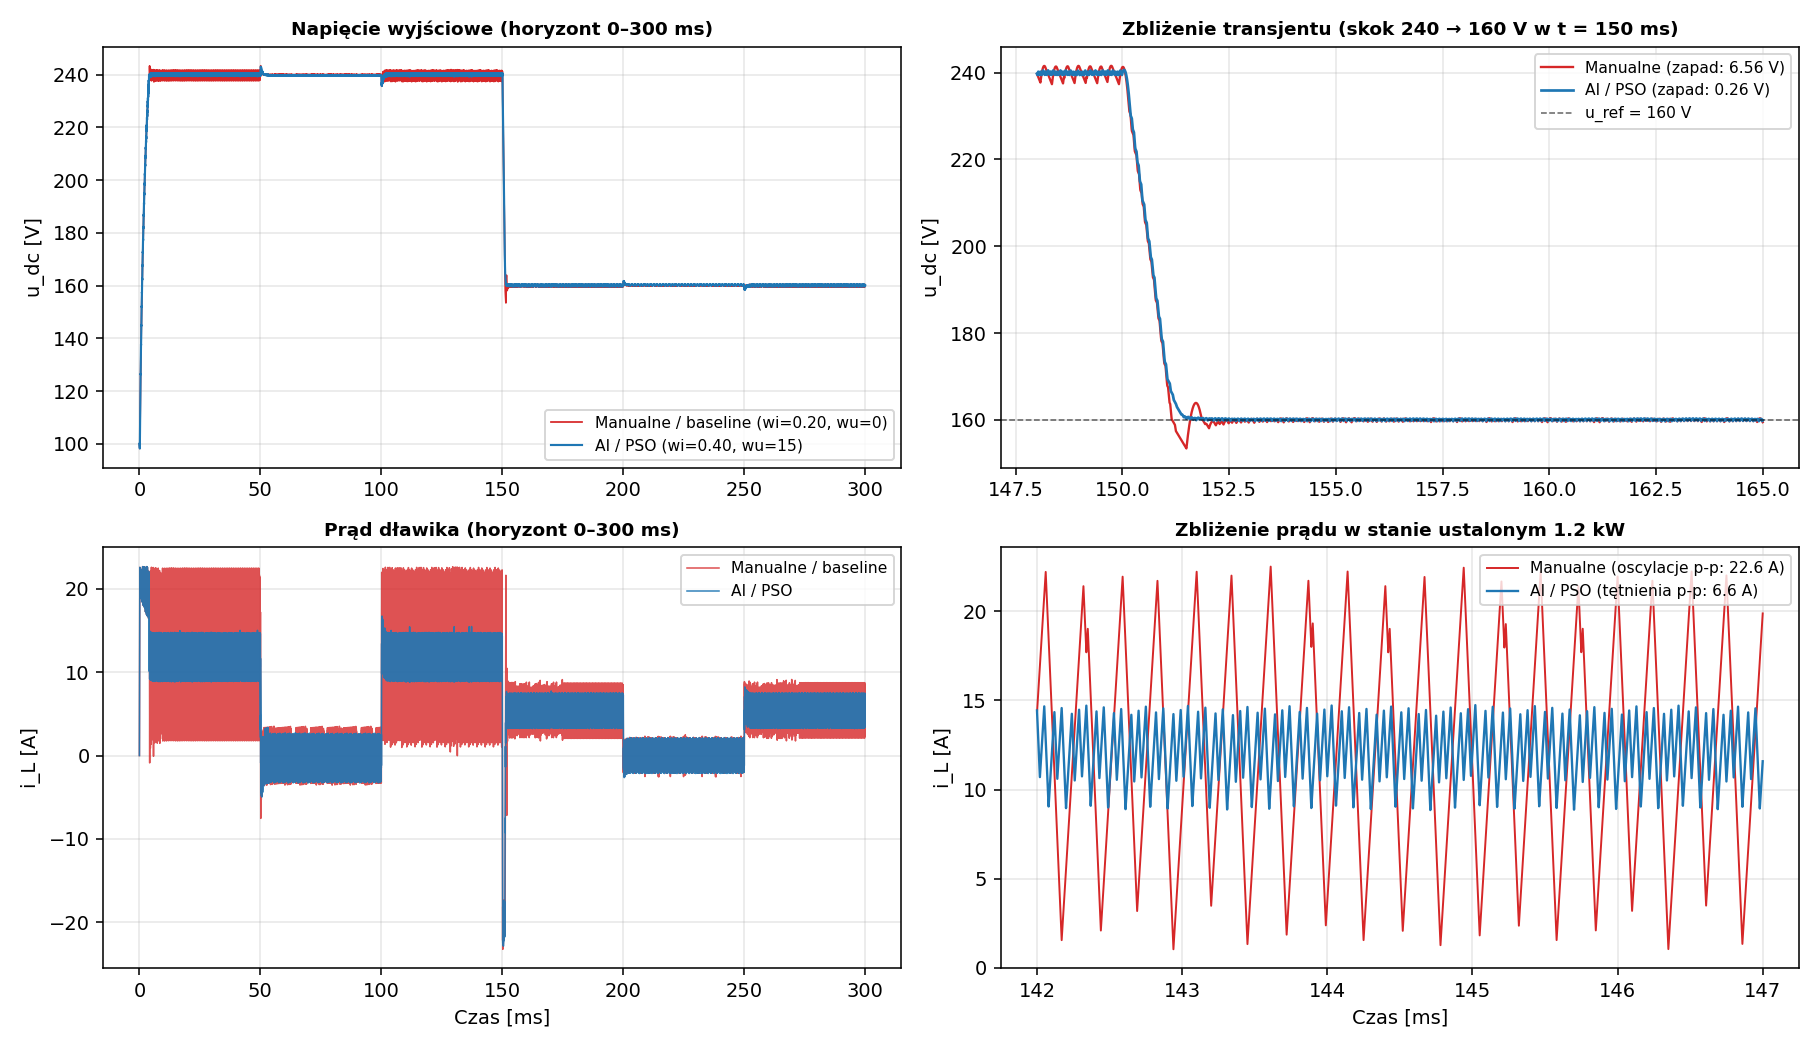
\includegraphics[width=\linewidth]{rysunki/porownanie_ai_vs_manual.png}
    \caption{Porównanie odpowiedzi czasowej przekształtnika: nastawy bazowe (linia czerwona) vs. nastawy nastrojone algorytmem PSO (linia niebieska). Widoczna całkowita eliminacja zapadu napięcia oraz drastyczna redukcja tętnień prądu w~stanie ustalonym.}
    \label{fig:ai-vs-manual}
\end{figure}

Optymalizacja metaheurystyczna przyniosła radykalną poprawę parametrów regulacji: zapad napięcia został zredukowany z~$6{,}56~\mathrm{V}$ do zaledwie $0{,}26~\mathrm{V}$ (poprawa o~$96{,}0\,\%$), a~tętnienia prądu dławika w~stanie ustalonym spadły z~$22{,}65~\mathrm{A}$ do $6{,}65~\mathrm{A}$ (poprawa o~$70{,}6\,\%$) dzięki wyprowadzeniu punktu pracy poza rejon oscylacji podharmonicznych ($w_i > 0{,}25$).

\section{Podsumowanie pracy}
\label{sec:podsumowanie}

\subsection{Realizacja celów pracy}
\label{subsec:realizacja-celow}

Wszystkie cele inżynierskie i~naukowe postawione w~rozdziale~\ref{sec:cel-zakres} zostały w~pełni zrealizowane:
\begin{enumerate}
    \item Opracowano kompletną, obiektową architekturę Bliźniaka Cyfrowego synchronicznego przekształtnika podwyższającego DC-DC w~języku Python, bazującą wyłącznie na bibliotece \texttt{numpy} i~wolną od ciężkich zależności komercyjnych.
    \item Zaimplementowano bezmodelowy algorytm sterowania przełączającego (MF-BB) oraz jego rozszerzenie o~człon trendu napięcia (Trend MF-BB) z~dyskretną filtracją sygnałów metodą Tustina.
    \item Przeprowadzono rygorystyczną walidację symulatora względem oprogramowania PSIM, osiągając zgodność zmiennych stanu na poziomie $0{,}05\,\%$ oraz potwierdzając poprawność równań testem odtworzeniowym (\emph{replay test}).
    \item Zintegrowano silnik symulacyjny z~autorskim algorytmem Optymalizacji Rojem Cząstek (PSO), formułując wielokryterialne funkcje celu uwzględniające jakość napięcia i~tętnienia prądu.
    \item Wdrożono dwutorową procedurę optymalizacji, która wyeliminowała zapady napięcia w~stanach przejściowych przy małej pojemności filtra ($C = 200~\mu\mathrm{F}$) i~wykazano jej wysoką odporność w~systematycznym badaniu wrażliwości.
\end{enumerate}

\subsection{Trudności napotkane podczas realizacji}
\label{subsec:trudnosci}

Podczas realizacji projektu rozwiązano szereg nietrywialnych problemów informatycznych i~symulacyjnych:
\begin{itemize}
    \item \textbf{Opóźnienie próbkowania ZOH i~kolejność zdarzeń:} Osiągnięcie idealnej zgodności z~symulatorem PSIM wymagało zamodelowania jednookresowego opóźnienia przetwornika ADC ($ZOH$ delay) oraz przyjęcia konwencji rejestracji stanu przed wykonaniem kroku fizyki.
    \item \textbf{Pułapka stanu przejściowego w~funkcjach celu:} Naiwne całkowanie błędu prądu na całym horyzoncie czasowym karało sterownik za wymuszone nasycenie prądu podczas rozruchu. Problem rozwiązano poprzez dekompozycję procedury na stan ustalony i~stan przejściowy.
    \item \textbf{Zjawisko fałszywego optimum przy twardej karze za zapad:} Wstępna definicja funkcji celu karząca wyłącznie zapad poniżej wartości zadanej powodowała sztuczne spowalnianie filtru napięcia przez PSO (do $157~\mathrm{Hz}$) kosztem późniejszego odbicia w~górę. Dopiero wprowadzenie kryterium całki kwadratu błędu (ISE) zharmonizowało kompromis pomiędzy szybkością a~gładkością lądowania.
\end{itemize}

\subsection{Wnioski końcowe}
\label{subsec:wnioski}

Przeprowadzone badania pozwalają na sformułowanie następujących wniosków końcowych:
\begin{enumerate}
    \item Standardowy ekosystem języka Python (CPython + NumPy) stanowi w~pełni dojrzałe, wydajne i~precyzyjne środowisko do tworzenia Bliźniaków Cyfrowych układów energoelektronicznych, oferując dokładność całkowicie równoważną dedykowanym narzędziom komercyjnym.
    \item Sterowanie bezmodelowe typu Bang-Bang (MF-BB) w~połączeniu z~członem trendu napięcia wykazuje doskonałe właściwości dynamiczne w~przekształtnikach o~zredukowanej pojemności filtra wyjściowego, skutecznie tłumiąc stany nieustalone.
    \item Dwutorowa optymalizacja metaheurystyczna z~wykorzystaniem algorytmu PSO eliminuje konieczność żmudnego, intuicyjnego strojenia parametrów regulatora, gwarantując powtarzalny dobór nastaw o~udowodnionej odporności na zmiany wag kryteriów optymalizacyjnych.
\end{enumerate}

\subsection{Kierunki dalszych prac}
\label{subsec:przyszlosc}

Naturalnymi kierunkami dalszego rozwoju projektu są:
\begin{itemize}
    \item Zrównoleglenie ewaluacji roju cząstek za pomocą modułu \texttt{multiprocessing} w~celu dalszego skrócenia czasu strojenia na wielordzeniowych stacjach roboczych.
    \item Rozszerzenie modeli symulacyjnych o~nieliniowości elementów pasożytniczych (zależność indukcyjności od prądu nasycenia rdzenia, charakterystyki temperaturowe tranzystorów GaN/SiC).
    \item Eksperymentalna weryfikacja wyznaczonych nastaw regulatora na fizycznym stanowisku laboratoryjnym z~mikrokontrolerem sygnałowym DSP / FPGA.
\end{itemize}
